\section{Problems with Existing Robotic Lawn Mowers}
Some commercially available robotic lawn mowers require a guard wire placed around the lawn. It can either be installed at the surface, and be held in place by pegs, or dug down below the surface. The guard wire must be routed around flower beds, bushes etc. as well, see \figref{fig:robomow}.\\\\
%
The use of the guard wire for guiding the mower back to the charging station presents another potential problem: in a garden with many restricted areas, the guard wire could get very long. Therefore the journey home could be longer, compared to a more direct route. This again uses more battery power, that could have been used for actually mowing the lawn instead.\\\\
%
This will be the motivation for the project: to avoid the work routing a wire around the garden, and as a bonus get more work done on a battery charge, by not wasting power following the wire home.\\\\

\begin{figure}[H]
\centering
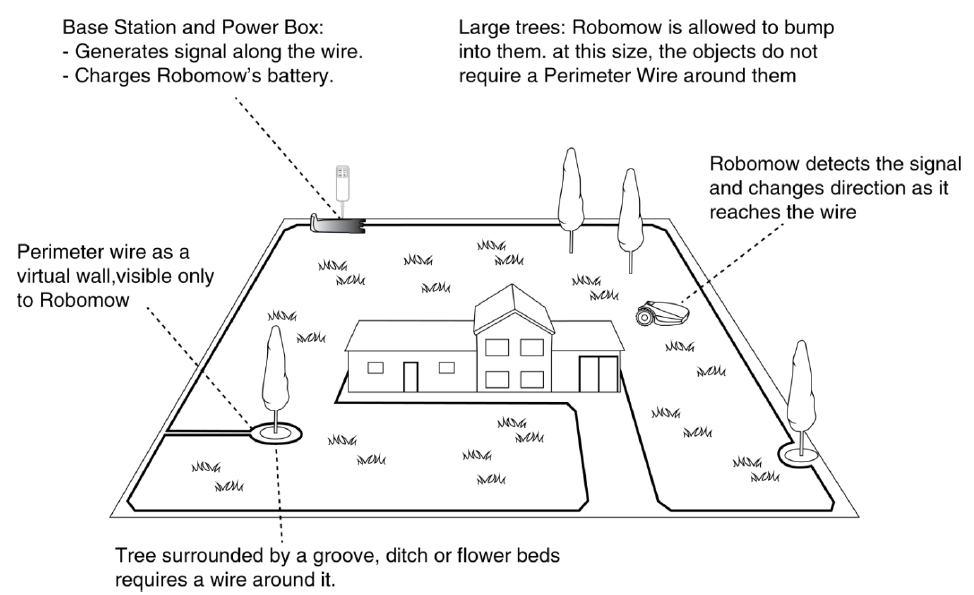
\includegraphics[scale=0.6]{figures/robomow.png} 
\caption{Guard wire installation [source:Robomow]}
\label{fig:robomow} 
\end{figure}
\noindent

Then, the next question is: what other solutions could be used to get the lawn mower to go where it has to go?
The solution of keeping track of where it is in real-time is examined in this project.